\documentclass{article}

\usepackage[utf8]{inputenc}
\usepackage{fancyhdr}
\usepackage{graphicx}
\usepackage{hyperref}
\usepackage[headheight=3cm]{geometry}


\title{\vspace{1.5cm}\\Documentation}
\author{\\
        \\
        Concerning software: \hspace{0.5cm} PyETL \&  DecubiTection \hspace{0.7cm} \\
        \\
        Submitted by : \hspace{1.5cm} Alex Jenke, Markus Fritzsche \\
        \\
        Submitted on: \hspace{1.65cm} February 06 2020 \hspace{2.05cm} \vspace{1.5cm}}
\date{}


\pagestyle{fancy}
\fancyhf{}
\rhead{\vspace{2cm} 
\includegraphics{images/logo2.png}\vspace{0.5cm} \\  }
\lhead{\vspace{2cm} 
\includegraphics{images/logo.png} \vspace{0.5cm} \hrule Zentrum für Medizinische Informatik}
\rfoot{\thepage}



\begin{document}
\pagenumbering{none}
\maketitle
\thispagestyle{fancy}
\setcounter{tocdepth}{2}
\tableofcontents
\newpage

\pagenumbering{arabic}
\section{Description}
This documentation describes the software: \textit{PyETL} \& \textit{DecubiTection}, a software transforming CSV data into an OMOP common data model and using machine learning to identify potential decubitus risks, regarding hospital patients.

The software is divided into three main systems: \textit{ETL process}, \textit{Machine Learning / Decubitus risk prediction} and \textit{Front-end}. 
Each system is able to run on its own and only depends on the results of the preceding subsystem stored in a database.

\begin{figure}[htbp]
\centerline{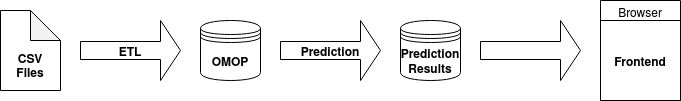
\includegraphics[width=1\linewidth]{images/DecubitusPipeline.png}}
\caption{Overview over the subsystems and their relations}
\label{fig:pipeline}
\end{figure}

There is the possibility to schedule the ETL-Process and the decubitus 
detection algorithm in a certain interval through a cron job. 
For this purpose, a Python script is provided which is able to create a cron job with the required parameters such as database host, password, etc.

\subsection{ETL process}
The purpose of the ETL-Process is to map medical data, provided by a set of CSV files formatted according to the specifications of §21 Paragraphs 4 and 5 KHEntgG, into the OMOP common data model (CDM).
This step is required, since the later described machine learning system learns and predicts, using data, gathered from an OMOP CDM. 

The ETL-Process requires certain preconditions. The CSV files are required to only contain valid and new data. Otherwise, the ETL-Process might fail or inconsistent data will be inserted into the OMOP database. 

The following explanation describes the ETL-Process for a single patient. 
In the first step, data from the \textit{FALL.csv} file gets extracted and will be inserted in the OMOP database, according to table \ref{etl-person}.
Since the provided data does not contain information about the patient's race and ethnicity, default values will be inserted. 
In case the patient's location is not already stored in the database, the ETL-Process will supplement this information, as depicted in table \ref{etl-location}.
If in two or more visits, the information differs, only the most up-to-date information will be inserted.
For every row in the FALL.csv file, a new visit will be inserted into VISIT\_OCCURRENCE as shown in table \ref{etl-visit}.
If the care site, the patient is currently located in, is not stored in the CARE\_SITE table, a new record is added, as illustrated in table \ref{etl-caresite}.

In the next step, all values - concerning the patient - from the \textit{LABOR.csv} file will be inserted, as depicted in table \ref{etl-labor}.
As the file only contains measurements, rows containing a different domain ID than "Measurement" will be skipped. 
If that happens, a warning will be printed onto STDERR. 
Similarly, the ETL-Process maps the data from \textit{MEASUREMENT.csv} to the database, as illustrated in table \ref{etl-measurement}.

The data from the \textit{ICD.csv} file is mapped as follows. If the domain ID of a row is an "Observation", a new observation will be inserted into OBSERVATION. 
If the value of "sekundaer\_kode" is empty, only one data record will be added as depicted in table \ref{etl-icd-observation}, in which case "ICD.icd\_kode" is mapped to observation\_source\_value.
If "sekundaer\_kode" is not empty, a second record will be added, where "ICD.sekundaer\_kode" is mapped to observation\_source\_value.

If the domain ID is a "Condition", instead of an "Observation", a new condition will be inserted in the database, as depicted by table \ref{etl-icd-condition}.
Similar to the previously described case, if a "sekundaer\_kode" is available, another record will be added. This is illustrated in table \ref{etl-icd-condition}. 
Additionally, if "lokalisation" is not empty, a new record will be inserted in the database, as shown in table \ref{etl-icd-location}.
The same applies if "diagnosesicherheit" is not empty, in which case the data is mapped as depicted in table \ref{etl-icd-diagnosensicherheit}.
Both records will be connected to the previously generated records through a fact relationship in both directions, as illustrated in table \ref{fact-relation}. 
If the domain id is neither "Condition" nor "Observation", the row will be skipped and a warning will be printed.

From \textit{OPS.csv}, the ETL-Process maps all procedures - concerning the patient - to the database, as illustrated in table \ref{etl-ops}.
Equally as described earlier, if a row contains a domain id, different from "Procedure", the row will be skipped and a warning will be printed.

%FALL.csv
\begin{table} [htbp]
\begin{tabular}{|l|l|}
 \hline
  \textbf{source column} & \textbf{destination column} \\
  \hline
  FALL.patienten\_nummer & PERSON.person\_id \\
  FALL.last\_record & PERSON.gender\_concept\_id \\
  FALL.geburtsjahr & PERSON.year\_of\_birth \\
  FALL.geburtsmonat & PERSON.month\_of\_birth \\
  "Unknown" & PERSON.race\_concept\_id \\
  "Not Hispanic" & PERSON.ethnicity\_concept\_id \\
  FALL.gender\_source\_value & PERSON.geschlecht \\
  \textit{LOCATION}.location\_id & PERSON.location \\
  \hline
\end{tabular}
\caption{Insert data from FALL.csv into table PERSON.}
\label{etl-person}
\end{table}

% LOCATION
\begin{table} [htbp]
\begin{tabular}{|l|l|}
  \hline
  \textbf{source column} & \textbf{destination column} \\
  \hline
  FALL.city & LOCATION.city \\
  FALL.zip & LOCATION.zip \\
  \hline
\end{tabular}
\caption{Insert a patient's location from FALL.csv to LOCATION.}
\label{etl-location}
\end{table}

\begin{table} [htbp]
\begin{tabular}{|l|l|}
  \hline
  \textbf{source column} & \textbf{destination column} \\
  \hline
  FAB.FAB & CARE\_SITE.care\_site\_name \\
  \hline
\end{tabular}
\caption{Insert a patient's visits to VISIT\_OCCURRENCE.}
\label{etl-visit}
\end{table}

% VISIT OCCURRENCE
\begin{table} [htbp]
\begin{tabular}{|l|l|}
  \hline
  \textbf{source column} & \textbf{destination column} \\
  \hline
  FALL.kh\_internes\_kennzeichen & VISIT\_OCCURRENCE.visit\_occurrence\_id \\
  FALL.aufnahmeanlass & VISIT\_OCCURRENCE.visit\_concept\_id \\
  FALL.aufnahmedatum & VISIT\_OCCURRENCE.visit\_start\_date \\
  FALL.entlassungsdatum & VISIT\_OCCURRENCE.visit\_end\_date \\
  "Visit derived from EHR record" & VISIT\_OCCURRENCE.visit\_type\_concept\_id \\
  FALL.aufnahmeanlass & VISIT\_OCCURRENCE.visit\_source\_value \\
  FALL.aufnahmegrund & VISIT\_OCCURRENCE.admitting\_source\_value \\
  FALL.entlassungsgrund & VISIT\_OCCURRENCE.discharge\_to\_source\_value \\
  \textit{CARE\_SITE}.care\_site\_id & VISIT\_OCCURRENCE.care\_site\_name \\
  \hline
\end{tabular}
\caption{Insert a new care site.}
\label{etl-caresite}
\end{table}

% LABOR -> MEASUREMENT
\begin{table} [htbp]
\begin{tabular}{|l|l|}
  \hline
  \textbf{source column} & \textbf{destination column} \\
  \hline
  LABOR.concept\_id & MEASUREMENT.measurement\_concept\_id \\
  LABOR.timestamp & MEASUREMENT.measurement\_date \\
  LABOR.timestamp & MEASUREMENT.measurement\_datetime \\
  "Lab Result" & MEASUREMENT.measurement\_type\_concept\_id \\
  LABOR.value & MEASUREMENT.value\_as\_number \\
  LABOR.concept\_id & MEASUREMENT.measurement\_source\_concept\_id \\
  LABOR.LOINC & MEASUREMENT.measurement\_source\_value \\
  LABOR.unit & MEASUREMENT.unit\_source\_value \\
  \hline
\end{tabular}
\caption{Insert measurement from LABOR.csv into MEASUREMENT.}
\label{etl-labor}
\end{table}

% MESSUNGEN -> MEASUREMENT
\begin{table} [htbp]
\begin{tabular}{|l|l|}
  \hline
  \textbf{source column} & \textbf{destination column} \\
  \hline
  MESSUNGEN.concept\_id & MEASUREMENT.measurement\_concept\_id \\
  MESSUNGEN.timestamp & MEASUREMENT.measurement\_date \\
  MESSUNGEN.timestamp & MEASUREMENT.measurement\_datetime \\
  "From physical examination" & MEASUREMENT.measurement\_type\_concept\_id \\
  MESSUNGEN.concept\_id & MEASUREMENT.measurement\_source\_concept\_id \\
  MESSUNGEN.LOINC & MEASUREMENT.measurement\_source\_value \\
  MESSUNGEN.value & MEASUREMENT.value\_as\_number \\
  MESSUNGEN.unit & MEASUREMENT.unit\_source\_value \\
  \hline
\end{tabular}
\caption{Insert measurement from MEASUREMENT.csv into MEASUREMENT.}
\label{etl-measurement}
\end{table}

%ICD.csv
\begin{table} [htbp]
\begin{tabular}{|l|l|}
  \hline
  \textbf{source column} & \textbf{destination column} \\
  \hline
  ICD.concept\_id & OBSERVATION.observation\_concept\_id \\
  FALL.aufnahmedatum & OBSERVATION.observation\_date \\
  "Observation recorded from EHR" & OBSERVATION.observation\_type\_concept\_id \\
  ICD.concept\_id & OBSERVATION.observation\_source\_concept\_id \\
  ICD.icd\_kode / ICD.sekundaer\_kode & OBSERVATION.observation\_source\_value \\
  \hline
\end{tabular}
\caption{Insert observation from ICD.csv into the OBSERVATION.}
\label{etl-icd-observation}
\end{table}

% LOCALISATION
\begin{table} [htbp]
\begin{tabular}{|l|l|}
  \hline
  \textbf{source column} & \textbf{destination column} \\
  \hline
  ICD.lokalisation & OBSERVATION.observation\_concept\_id \\
  FALL.aufnahmedatum & OBSERVATION.observation\_date \\
  "Observation recorded from EHR" & OBSERVATION.observation\_type\_concept\_id \\
  ICD.lokalisation & OBSERVATION.observation\_source\_value \\
  ICD.lokalisation & OBSERVATION.value\_as\_string \\
  \hline
\end{tabular}
\caption{Insert information about the location from 
    ICD.csv to OBSERVATION.}
\label{etl-icd-location}
\end{table}

% FACT RELATIONSHIP
\begin{table} [htbp]
\begin{tabular}{|l|l|}
  \hline
  \textbf{source column} & \textbf{destination column} \\
  \hline
  \textless table1\textgreater & FACT\_RELATIONSHIP.domain\_concept\_id\_1 \\
  \textit{\textless table1\textgreater}.observation\_id & FACT\_RELATIONSHIP.fact\_id\_1 \\
  \textless table2\textgreater & FACT\_RELATIONSHIP.domain\_concept\_id\_2 \\
  \textit{\textless table2\textgreater}.observation\_id & FACT\_RELATIONSHIP.fact\_id\_2 \\
  "Finding associated with/Associated with finding" & FACT\_RELATIONSHIP.relationship\_concept\_id \\
  \hline
\end{tabular}
\caption{Connect two entries through a fact relation.}
\label{fact-relation}
\end{table}

% diagnosensicherheit
\begin{table} [htbp]
\begin{tabular}{|l|l|}
  \hline
  \textbf{source column} & \textbf{destination column} \\
  \hline
  ICD.diagnosensicherheit & OBSERVATION.observation\_concept\_id \\
  FALL.aufnahmedatum & OBSERVATION.observation\_date \\
  "Observation recorded from EHR" & OBSERVATION.observation\_type\_concept\_id \\
  ICD.diagnosensicherheit & OBSERVATION.observation\_source\_value \\
  ICD.diagnosensicherheit & OBSERVATION.value\_as\_string \\
  \hline
\end{tabular}
\caption{Insert information about the diagnostic reliability from 
    ICD.csv to OBSERVATION.}
\label{etl-icd-diagnosensicherheit}
\end{table}

% CONDITION OCCURRENCE
\begin{table} [htbp]
\begin{tabular}{|l|l|}
  \hline
  \textbf{source column} & \textbf{destination column} \\
  \hline
  ICD.concept\_id & CONDITION\_OCCURRENCE.condition\_concept\_id \\
  FALL.aufnahmedatum & CONDITION\_OCCURRENCE.condition\_start\_date \\
  FALL.aufnahmedatum & CONDITION\_OCCURRENCE.condition\_start\_datetime \\
  ICD.diagnoseart & CONDITION\_OCCURRENCE.condition\_type\_concept\_id \\
  ICD.concept\_id & CONDITION\_OCCURRENCE.source\_concept\_id \\
  ICD.icd\_kode/ICD.sekundaer\_kode & CONDITION\_OCCURRENCE.source\_value \\
  \hline
\end{tabular}
\caption{Insert conditions from ICD.csv to CONDITION\_OCCURRENCE.}
\label{etl-icd-condition}
\end{table}

% OPS.csv
\begin{table} [htbp]
\begin{tabular}{|l|l|}
  \hline
  \textbf{source column} & \textbf{destination column} \\
  \hline
  OPS.concept\_id & PROCEDURE\_OCCURRENCE.procedure\_occurrence\_id \\
  OPS.ops\_datum & PROCEDURE\_OCCURRENCE.procedure\_date \\
  OPS.ops\_datum & PROCEDURE\_OCCURRENCE.procedure\_datetime \\
  "Procedure recorded as diagnostic code" & PROCEDURE\_OCCURRENCE.procedure\_type\_concept\_id \\
  OPS.ops\_kode & PROCEDURE\_OCCURRENCE.procedure\_source\_value \\
  OPS.concept\_id & PROCEDURE\_OCCURRENCE.procedure\_source\_concept\_id \\
  \hline
\end{tabular}
\caption{Insert procedures from OPS.csv into PROCEDURE\_OCCURRENCE.}
\label{etl-ops}
\end{table}

\newpage
\subsection{Decubitus Risk Prediction}
The decubitus risk prediction is provided by a neural network, trained on patient data of the OMOP CDM. 
The network takes a number of clinical findings as input and predicts binary the risk of the patient developing a pressure ulcer in the near future.
The specific findings used as input are determined by selecting the unique concept ids from the database which describe the patient's condition at the time a pressure ulcer is diagnosed.
Therefore only findings are selected that could possibly be connected to the risk of developing a decubitus.

In the training process, old patient data is sampled at different moments pairing the information on the patient's condition given at this point and the binary label whether a pressure ulcer will be diagnosed within the next n dates contained in the database.
N is a number to be configured prior to the training.
The sampled data is split into a testset and a trainset.
The network is trained only on the trainset, therefore the testset contains new unseen samples on which the network can be evaluated.

Once a neural network is trained on the trainset, validated on the testset and the classification threshold is selected, it can be loaded into the actual prediction pipeline.
The Pipeline takes the latest patient data from the OMOP CDM as input and calculates the decubitus risk prediction. 
Afterwards, using gradient backpropagation, the Pipeline determines the importance of the different inputs to the calculated prediction.
The most important clinical findings are filtered to reject meaningless Information and the top ten remaining facts are stored together with the prediction, to be displayed in the front-end.

\subsection{Front-End}

The front-end is a web application, running on a dedicated server, reachable only from the network of the medical institution. 
The patient data is protected by a login page, requiring a valid username and password. 
The data is extracted from the database, where the results of the decubitus risk detection pipeline are stored. 
The patient data is illustrated inside a table, where patients, potentially developing a decubitus are marked in red. 
The results can be downloaded and printed as a PDF file. 
Necessary parameters e.g. database connection settings can be configured as command line parameters on startup of the application. 
%\newpage

\section{Risk Analysis}
As shown in Table \ref{risks} four major risk classes are considered. 
Firstly data loss or manipulation due to bugs, secondly the nonavailability of the service, thirdly attacks by an unauthorized person and lastly the risks of wrong patient treatment due to the software.

\begin{table}[htbp]
\begin{tabular}{|c|c|c|c|}
	\hline
	 &\textbf{ Risk Description} & \textbf{Risk Likelihood} & \textbf{Risk Severity}\\
	\hline
    \hline
    %0 & nur für Informatiker & prabably & over 9000\\
    %\hline
    %\hline
    % data deletion manipulation by bugs
	1 & Patient data gets deleted/modified & low & high \\
	& by a bug in the front-end &&\\
	\hline
	2 & Patient data gets deleted/modified & high & high \\
	& by a bug in the ETL process &&\\
	\hline
	3 & Patient data gets deleted/modified & low & high \\
	& by a bug in the decubitus prediction back-end &&\\
	\hline
	4 & Data of decubitus prediction gets deleted/modified & medium & medium \\
	& by a bug in the front-end &&\\
	\hline
	5 & Data of decubitus prediction gets deleted/modified & low & medium \\
	& by a bug in the ETL process &&\\
	\hline
	6 & Data of decubitus prediction gets deleted/modified & high & medium \\
	& by a bug in the decubitus prediction back-end &&\\
	\hline
	\hline
	% dos 
	7 & The front-end is unavailable due to a dos attack & low & low \\
	\hline
	\hline
	% data manipulation by person
	8 & Unauthorized person tries to delete/manipulate & medium & high \\
	& data via the front-end & & \\
	\hline
	9 & Unauthorized person tries to get & medium & high \\
	& access to patient data via the front-end & & \\
	\hline
	\hline
	% effect on treatment
	10 & Patient is erroneously treated & middle & middle \\
	& due to the decubitus prediction && \\
	\hline
    11 & Patient is erroneously not treated  & middle & high \\
	& due to the decubitus prediction && \\
	\hline
\end{tabular}
\caption{Risk analysis}
\label{risks}
\end{table}

In the first risk, patient data in the OMOP database gets deleted or modified by a bug in the front-end. 
The severity of this risk is high because the correctness of the patient data is crucial and the data in the database in will not be checked on its correctness once it is inserted.  
The likelihood of this happening is low because the front-end never needs to write into the OMOP database and therefore the possibility of changing the data can be minimized by using only relevant read rights on database access.

In the second risk, patient data in the OMOP database gets deleted or modified by a bug in the ETL-Process. 
The severity of this risk is high because the correctness of the patient data is crucial and the data in the database in will not be checked on its correctness once it is inserted.  
The likelihood of this happening is high because this processes task is to translate the data from CSV files to an OMOP Database, bugs and errors in the implementation are possible.
Therefore the process needs to be tested to ensure the correctness of the implementation.

In the third risk, patient data in the OMOP database gets deleted or modified by a bug in the decubitus prediction back-end. 
The severity of this risk is high because the correctness of the patient data is crucial and the data in the database will not be checked on its correctness once it is inserted.  
The likelihood of this happening is low because the back-end never needs to write into the OMOP database and therefore the possibility of changing the data can be minimized by using only relevant read rights on database access.

In the fourth risk, data of the decubitus prediction gets deleted or modified by a bug in the front-end.
The severity of this risk is medium because the correctness of the data is crucial to the functionality of the software, but the software is not crucial to the workflow in a hospital.
The likelihood of this happening is medium because the front-end is responsible for the correct display of the information. Therefore unwanted modification of the data is possible and must be excluded by testing.
The likelihood of data deletion is low because the front-end never needs to write on the data and therefore the possibility of deletion can be minimized by using only relevant read rights on access.

In the fifth risk, data of the decubitus prediction gets deleted or modified by a bug in the ETL-Process.
The severity of this risk is medium because the correctness of the data is crucial to the functionality of the software, but the software is not crucial to the workflow in a hospital.
The likelihood of this happening is low because the ETL-Process is independent of the decubitus detection and only severe bugs or errors would lead to data deletion/modification in an completely separate database.

In the sixth risk, data of the decubitus prediction gets deleted or modified by a bug in the decubitus prediction back-end.
The severity of this risk is medium  because the correctness of the data is crucial to the functionality of the software, but the software is not crucial to the workflow in a hospital.
The likelihood of this happening is high because the prediction is generated in the back-end and errors are possible. 
Therefore testing and evaluation of the prediction is needed.

In the seventh risk, the front-end and thus the data on decubitus prediction is not available due to an attack overloading the providing back-end. 
The severity of this risk is low  because the availability of this service is not crucial to the workflow in a hospital.
This type of attack is one of the easiest ways to prevent the software's functionality, nevertheless, the likelihood is classified as low  because the front-end will only be available within the hospital's intranet. 
Therefore an attacker would be required to act inside a controlled network where he would easily be spotted and the attack could be ended.

In the eighth risk, an unauthorized person tries to manipulate/delete data via the front-end.
The severity of this risk is high  because the correctness of the data is crucial and deliberate modification could lead to critical endangerment of patients.
The likelihood is medium due to the fact that patient data front-ends are an easy target to manipulate the displayed data.
Therefore the access to the front-end needs to be protected by a password authentication.
Further, the front-end only provides read access on the displayed information and therefore no data in the database can be changed. 
Manipulations on the displayment of the data can be reverted by reloading the page.

In the ninth risk, an unauthorized person tries to access patient data via the front-end.
The severity of this risk is high  because patient data is highly confidential.
The likelihood is medium due to the fact that patient data front-ends are the first target on acquirement of patient data.
Therefore the access to the front-end needs to be protected by a password authentication.
Further, the front-end only provides selected patient data, e.g. the name, age, possibility of developing a decubitus and the top ten clinical findings leading to the decubitus prediction.

In the tenth risk, a patient gets erroneous treated to prevent the development of a decubitus.
The severity of this risk is medium due to the possibility of medicamental treatment leading to unnecessarily side effects. However, drug administration should always be medically questioned.
In addition, further measures, such as frequent repositioning, do not lead to any far-reaching impairment of the patient.
The risk of an erroneously treatment only based on the software is possible but, as emphasized, the software should only be used as a guide, including verifying the prediction using the top ten clinical findings leading to the prediction. Therefore the likelihood is medium.

In the eleventh risk, a patient gets erroneously not treated leading to the development of a decubitus.
The severity of this risk is high due to the far-reaching impairment of the patient.
The likelihood is medium as the risk of a faulty refraining from treatment only based on the software is possible but, as emphasized, the software should only be used as a guide and the risk assessment should remain in the doctor's responsibility.
%\newpage

\section{Quality Management} 
The software is developed according to the waterfall model.
\begin{itemize}
\item In the first step the task was analyzed and requirements for the software were documented.

\item Secondly the software structure was designed. 
In this step, the software was split into the three subsections: ETL-Process, Prediction-Pipeline, and front-end.
Interfaces, in form of database structures, were defined. 

\item In the third step, the sub-modules were implemented separately.

\item In the fourth step, the sub-modules were firstly tested independently and afterward the complete pipeline was evaluated.

\item The last step, the commissioning is prepared but not executed.

\end{itemize}
On completion of a step the fulfillment of the requirements of the preceding step were verified.
On implementation the sub-modules were split into smaller tasks, which were implemented and tested on its own, followed by a system test verifying the correct operation of the task in the complete system. 

%\newpage

\section{Software Life-cycle Processes}
\subsection{Requirements}
The following requirements for the software were identified:
\begin{itemize}
    \item The software transforms CSV files containing standardized patient data according to §21 Paragraph 4 and 5 KHEntgG into an OMOP CDM.
    \item The software can be configured to perform the transformation periodically.
    \item The software provides a prediction based on patient data of the patients risk developing a pressure ulcer (decubitus).
    \item The prediction on the risk of decubitus development can be verified on provided reasons leading to the classification.
    \item The generated prediction can be displayed in a web browser.
    \item The access to the patient data via the web browser is protected by a password authentication.  
\end{itemize}

\subsection{Tests}
The sub-modules of the software are tested independently due to the fact they only interact via defined interfaces in form of database entries.
Therefore only the correctness from one interface to another is tested.

In addition, one complete run from CSV to front-end is performed to ensure the correct interaction via the interfaces.

\subsubsection{ETL-Process}
The different functions of the ETL-Process are tested by unit tests.
Further, the complete sub-module is tested by inserting a set of CSV files into the OMOP CDM and checking the database content to contain the expected data.

\subsubsection{Decubitus Risk Prediction}
The decubitus risk prediction is based on a neural network, therefore the prediction can only be tested on test data. 
The F1-Score, recall, and precision are used to numerically evaluate the results.
Further, the returned top ten clinical findings are evaluated via visual inspection of the results. 

\subsubsection{Front-End}
The front-end was tested visually by displaying known data and checking the visualization for correctness.


\subsection{Change Management}
Updates for the subsections of the software can be deployed independently.
Therefore the change management for each segment needs to be analyzed separately.
This enables the fast deployment of bug fixes because only the affected sub-module needs to be updated, tested and deployed. 

\subsubsection{ETL-Process}
If the ETL-Process is updated it will be validated on test data.
Afterward it can be deployed.
The deployment simply consists of the replacement of affected Python files.
This can easily be done by using a versioning system like git. 
If a versioning system is used, the deployment only consists of the provider pushing the newest version and the customer pulling the newest version.

However, it should be noted that data already entered in the OMOP CDM will not be updated retroactively.
Meaning, erroneously data in the database can only be fixed by deleting affected entries and inserting it as a set of CVS files into the updated ETL-Process.

\subsubsection{Decubitus Risk Prediction}
The update routine of the decubitus risk prediction can be split into two different cases.

In the first case, the update fixes a bug in the prediction pipeline. 
A bug is detected and fixed in the code, followed by testing of the sub-module.
Afterward the new version can be deployed similar to the ETL-Process.

In the second case, the neural network (NN) is updated.
Assuming the trainset is extended by new data the NN can be retrained on the new data.
If the new network achieves better test results than the old version it can be deployed.
For this purpose, the file that defines the NN is updated and deployed similar to the ETL-Process.


\subsubsection{Front-End}
If the front-end is updated, it will be validated through usability-tests\footnote{tests, where one or more developers validate the software through simply using it}, where the patient data is replaced with dummy data. 
If these tests succeed, the sub-module can be deployed by replacing the contained Python, CSS, JavaScript and HTML files.
As the front-end only requires reading access to the database, two instances of different versions can run separately. 
Hence, if a newer version contains bugs or missing functionality, one can fall back to the previous version and report the issue to the developers.
Therefore the front-end offers high availability. 



%The purpose of our product is to predict potential decubitus patients with aid of patient specific medical records. In order to achieve a system of this capability, many steps are required.
%We need to constantly convert data into the OMOP CDM, evaluate the data and illustrate the results on doctors or medical assistants, hence they are able to treat the patients correctly. 

%\subsection{Development of an ETL Process}
%The first step of the product is to convert our standardized data into the OMOP CDM. 
%In order to achieve that, we write a Python framework, reading the data of the input CSV files, connect to the required database and saves the converted data.

%\subsection{Evaluation of the data}
%To achieve the best possible results, we focus on a deep learning approach, hence our system learns from real data, how likely it is that a patient suffers on decubitus. 
%Secondarily we work on a pure statistically approach as base line.
%If the second approach ends up more reliable, we discard the deep learning approach.
%As training data, we use a set of medical records from dummy patients.
%Unfortunately we don't have the opportunity to train on real patient data, as OHDSI don't offer real data of patients who actually suffered from decubitus. 

%\subsection{Building the app}
%We build a simple web python application for the use of our medical device.
%This app is possible to schedule when the ETL process should restart, configure the database settings and illustrate the results of the patient evaluation. 

%\newpage

\section{Usability}
\subsection{Front-End}
For the front-end, we chose a web application, written in Python. 
We did not offer the choice for a different approach in the questionnaire, as a web application offers the most flexibility. 
The admin is able to configure the desired information, and the actual users of the front-end do not need to concern about it.
Another advantage is that no additional software has to be installed on the computers in the medical institution. 
Front-end users only need to open an arbitrary internet browser and navigate to the front-end page. 
Furthermore, in case the front-end needs to be updated, one has not to update the software on each computer. 

\subsubsection{Design}
We offered various design options for the front-end in the questionnaire. 
In the end, the most popular design is illustrated in \ref{fig:gray-color}. 
Potential decubitus patients are marked in red, showing the user that he requires additional attention.
If the user clicks on a red marked patient, a text appears, describing why DecubiTection decided that the patient may develop a decubitus. 
On the other hand, if the user clicks on a gray marked patient, a text appears that no risks concerning decubitus are found, but that there may be still a residual risk, as the detection algorithm is not perfectly accurate. 
In case, the user is confused by the front-end, we included a help button, illustrated in \ref{fig:help}, which describes how to use the software. 

\begin{figure}[htp]
    \centering
    \frame{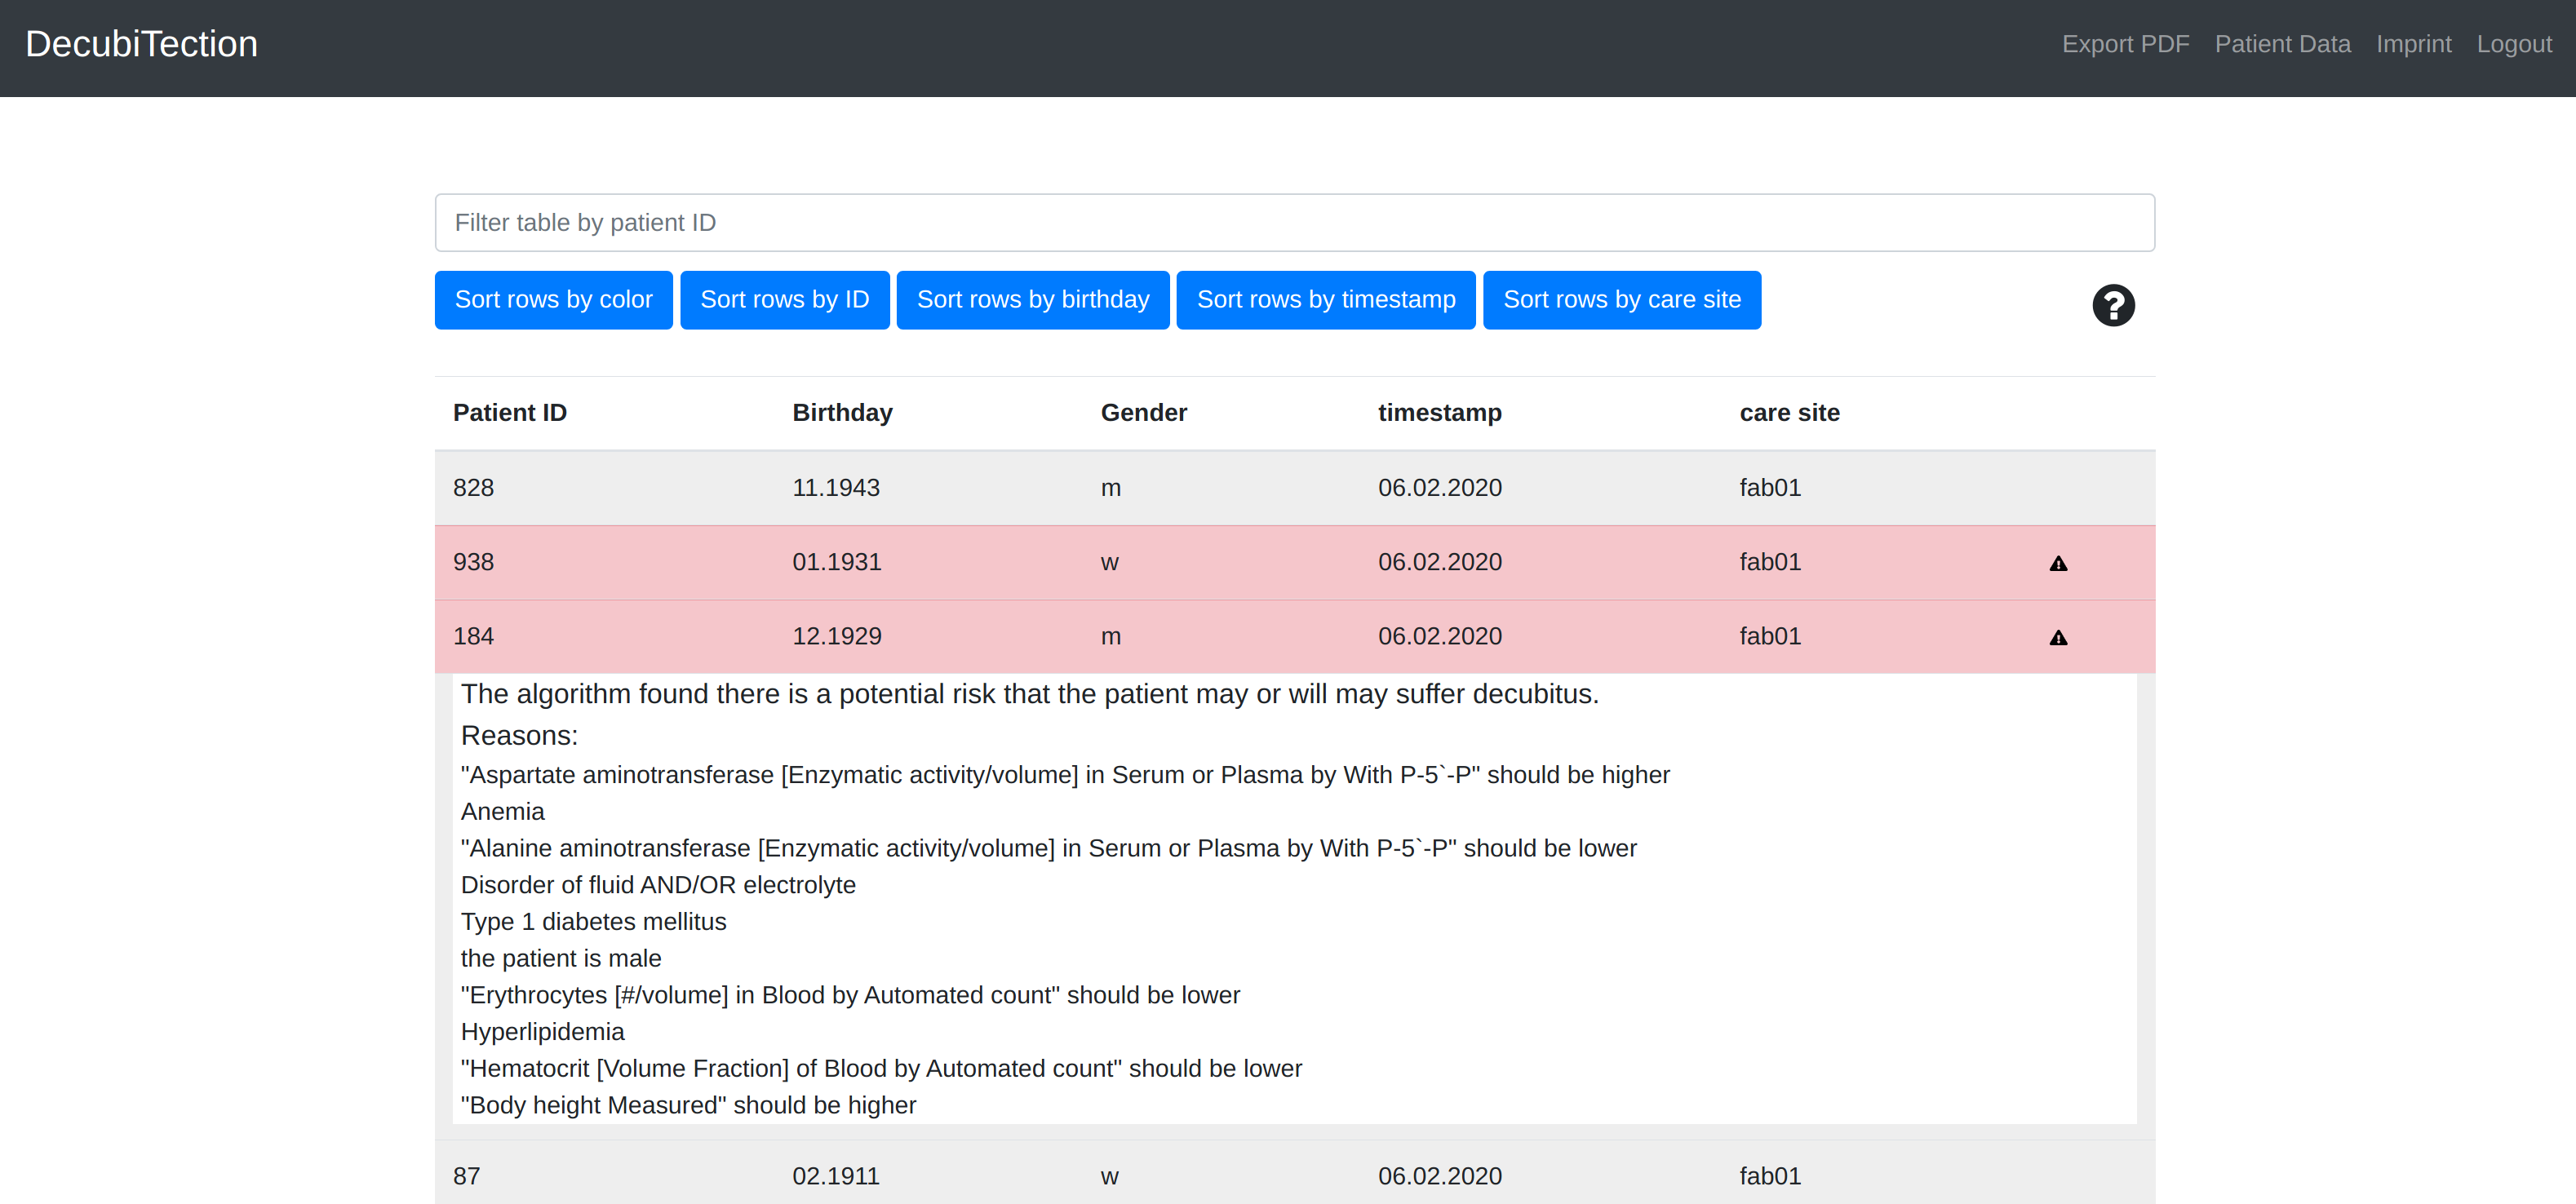
\includegraphics[width=15cm]{images/gray.png}}
    \caption{Most popular color theme of the front-end.}
    \label{fig:gray-color}
\end{figure}

\begin{figure}[htp]
    \centering
    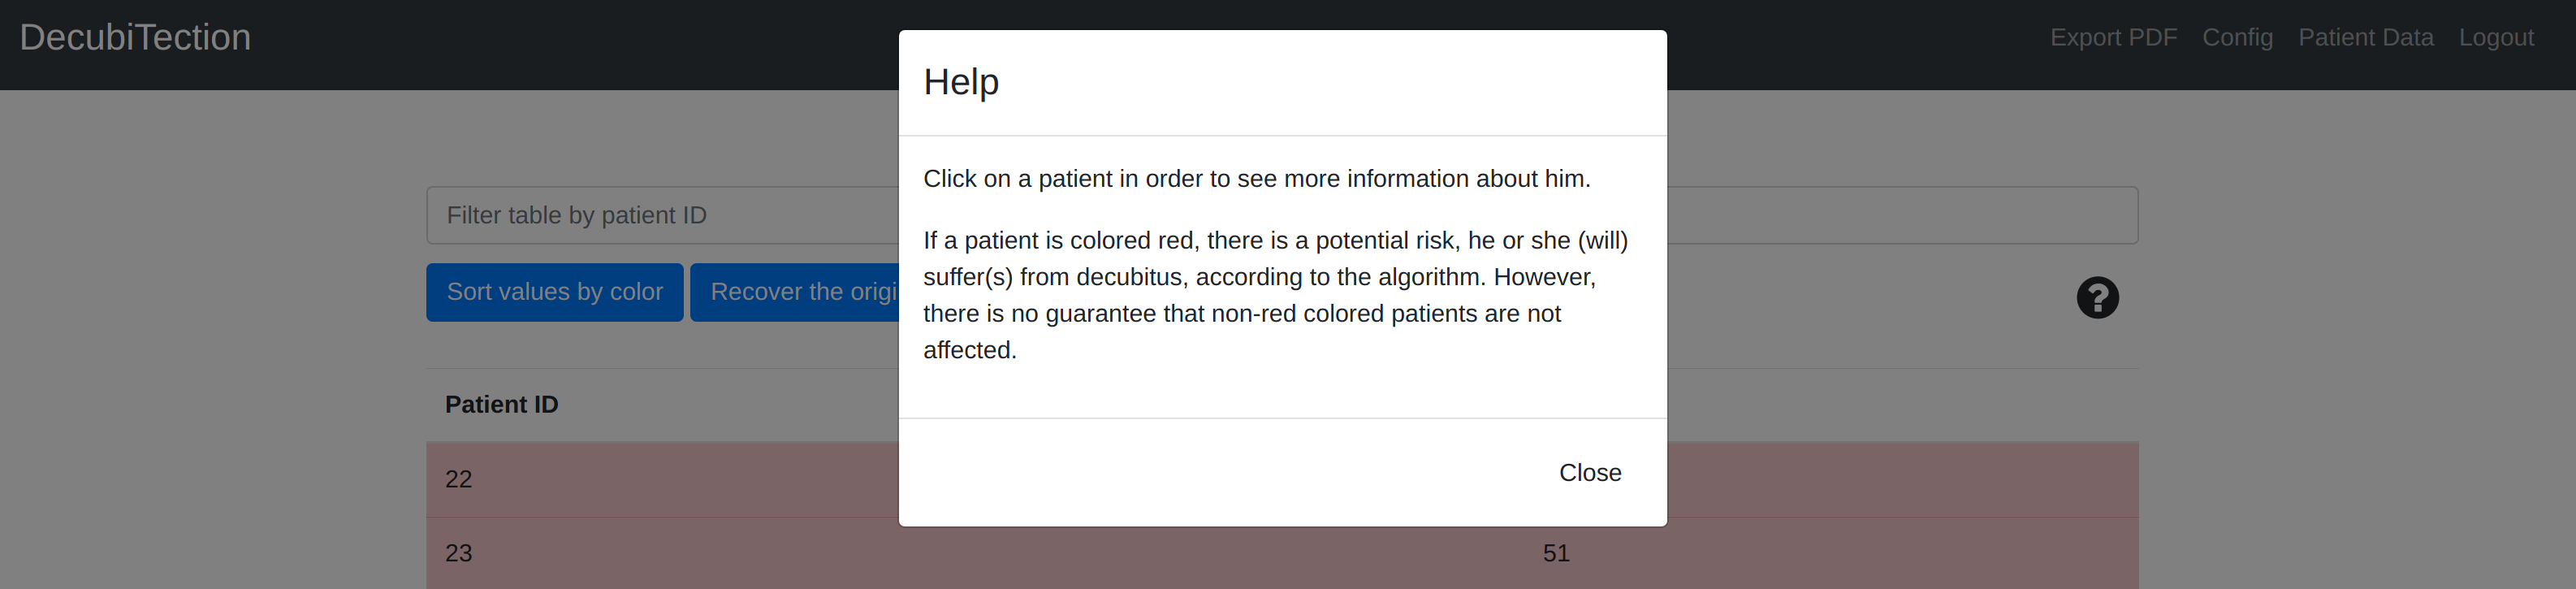
\includegraphics[width=15cm]{images/help.png}
    \caption{The help page of DecubiTection.}
    \label{fig:help}
\end{figure}

Though a web application brings many advantages, it contains a major disadvantage as well. 
Everyone inside the local network of the medical institution is able to access the front-end. 
We solved this by adding an authentication system, requiring valid credentials in order to access the front-end, depicted in \ref{fig:login}.
This decision matches the results of the questionnaire. 

\begin{figure}[htp]
    \centering
    \frame{
\includegraphics[width=15cm]{images/login.png}}
    \caption{The login page of DecubiTection.}
    \label{fig:login}
\end{figure}

\subsubsection{Content}
The results of the questionnaire showed that as general information, at least the patient ID and the birthday of the patient are required. 
Additionally, we added the patient's gender and the care-site, the patient is currently located in. 
In the front-end, one can filter patients by their ID and sort them by background colors. 
We included the option to save the results as PDF file as well. 
Hence a user is able to print the results. 

\subsubsection{Configuration}
There are different opinions, whether the front-end should include a configuration page e.g. for database credentials. 
We decided to not included such a page since it is not the front-end's users task to configure the software. 
In the current state, only an admin is able to configure the database settings and the credentials for authentication. 

\subsection{Back-End}
The cron job for the ETL-Process and the detection algorithm needs to be configured, according to several parameters. 
According to the results of the questionnaire, it is sufficient to include these parameters through command line parameters, e.g. \textit{python3 cron.py --db\_port=1234 --db\_host=localhost}.
Furthermore, the questionnaire showed the necessity for the following parameters:

\begin{itemize}
	\item cron interval
	\item for the database:
	\subitem username
	\subitem password
	\subitem host
	\subitem port
	\item location of the CSV files
\end{itemize}

Log files can be generated by redirecting the output of the software 
into a log-file. 

\section{Dependencies}
\subsection{ETL-Process}
The submodule requires:
\begin{itemize}
    \item python $>$= 3.6
    \item psycopg2 $>$= 2.8.4
    \item pandas $>$= 0.25.3
    \item numpy $>$= 1.17.4
    \item tqdm $>$= 4.38.0
    \item python-crontab $>$=2.4.0
\end{itemize}

\subsection{Decubitus Risk Prediction}
The submodule requires:
\begin{itemize}
    \item python $>$= 3.6
    \item psycopg2 $>$= 2.8.4
    \item torch $>$= 1.4.0
    \item numpy $>$= 1.17.4
    \item tensorboardX $>$= 1.9
    \item matplotlib $>$= 3.2.0rc1
    \item tqdm $>$= 4.38.0
\end{itemize}

\subsection{Front-End}
The submodule requires:
\begin{itemize}
    \item python $>$= 3.6
    \item psycopg2 $>$= 2.8.4
    %\item pandas $>$= 0.25.3
    %\item numpy $>$= 1.17.4
    \item flask $>$=1.1.1
    \item fpdf $>$=1.7.2
\end{itemize}
\end{document}